\section{Heartbeat sensor}
\begin{figure}[H]
    \centering
    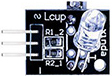
\includegraphics[angle=0, keepaspectratio=true, scale=1, width=200px, height=200px]{images/heartbeat.jpg}
    %\caption{Caption}
\end{figure}
\subsection*{Description}
The heartbeat sensor module consists of an Infrared (IR) LED and a phototransistor (photosensor).
\subsection*{Pin mapping}
This pin mapping corresponds to the pins from left to right with the module pins facing towards you.
\begin{table}[H]
    \centering
    \begin{tabular}{|c|c|c|c|c|}
    \hline
    Index &Label &Type &Name &Description\\ \hline
    0 &S &Analog output &A0 &\\ \hline
    1 & &Source voltage &$V+$ &Module source voltage ($5V$)\\ \hline
    2 &- &Ground &GND &Ground\\ \hline
    \end{tabular}
    %\caption{Caption}
    %\label{tab:my_label}
\end{table}
\subsection*{Operation}
The output voltage at the analog pin (A0) is related to the magnetic field strength near the sensor. When there is no magnetic field, this output is half the supply voltage. As the ESP32 ADC can only measure voltages between 0V to 3.3V, it is recommended to supply the module with 3.3V (for larger swing). Applying a magnetic field oriented in one direction will cause the analog output voltage to be increase, the other direction will cause the voltage to decrease.
\subsection*{Code}
Refer to listing \ref{python_heartbeat}.
%\lstinputlisting[caption=test]{laser.py}